\documentclass{beamer}
\mode<presentation>
\usepackage{amsmath,amssymb,mathtools}
\usepackage{textcomp}
\usepackage{gensymb}
\usepackage{adjustbox}
\usepackage{subcaption}
\usepackage{enumitem}
\usepackage{multicol}
\usepackage{listings}
\usepackage{url}
\usepackage{graphicx} % <-- needed for images
\def\UrlBreaks{\do\/\do-}

\usetheme{Boadilla}
\usecolortheme{lily}
\setbeamertemplate{footline}{
  \leavevmode%
  \hbox{%
  \begin{beamercolorbox}[wd=\paperwidth,ht=2ex,dp=1ex,right]{author in head/foot}%
    \insertframenumber{} / \inserttotalframenumber\hspace*{2ex}
  \end{beamercolorbox}}%
  \vskip0pt%
}
\setbeamertemplate{navigation symbols}{}

\lstset{
  frame=single,
  breaklines=true,
  columns=fullflexible,
  basicstyle=\ttfamily\tiny   % tiny font so code fits
}

\numberwithin{equation}{section}

% ---- your macros ----
\providecommand{\nCr}[2]{\,^{#1}C_{#2}}
\providecommand{\nPr}[2]{\,^{#1}P_{#2}}
\providecommand{\mbf}{\mathbf}
\providecommand{\pr}[1]{\ensuremath{\Pr\left(#1\right)}}
\providecommand{\qfunc}[1]{\ensuremath{Q\left(#1\right)}}
\providecommand{\sbrak}[1]{\ensuremath{{}\left[#1\right]}}
\providecommand{\lsbrak}[1]{\ensuremath{{}\left[#1\right.}}
\providecommand{\rsbrak}[1]{\ensuremath{\left.#1\right]}}
\providecommand{\brak}[1]{\ensuremath{\left(#1\right)}}
\providecommand{\lbrak}[1]{\ensuremath{\left(#1\right.}}
\providecommand{\rbrak}[1]{\ensuremath{\left.#1\right)}}
\providecommand{\cbrak}[1]{\ensuremath{\left\{#1\right\}}}
\providecommand{\lcbrak}[1]{\ensuremath{\left\{#1\right.}}
\providecommand{\rcbrak}[1]{\ensuremath{\left.#1\right\}}}
\theoremstyle{remark}
\newtheorem{rem}{Remark}
\newcommand{\sgn}{\mathop{\mathrm{sgn}}}
\providecommand{\abs}[1]{\left\vert#1\right\vert}
\providecommand{\res}[1]{\Res\displaylimits_{#1}}
\providecommand{\norm}[1]{\lVert#1\rVert}
\providecommand{\mtx}[1]{\mathbf{#1}}
\providecommand{\mean}[1]{E\left[ #1 \right]}
\providecommand{\fourier}{\overset{\mathcal{F}}{ \rightleftharpoons}}
\providecommand{\system}{\overset{\mathcal{H}}{ \longleftrightarrow}}
\providecommand{\dec}[2]{\ensuremath{\overset{#1}{\underset{#2}{\gtrless}}}}
\newcommand{\myvec}[1]{\ensuremath{\begin{pmatrix}#1\end{pmatrix}}}
\let\vec\mathbf
% ---------------------

\title{Matgeo Presentation - Problem 1.10.19}
\author{ee25btech11056 - Suraj.N}

\begin{document}

\begin{frame}
  \titlepage
\end{frame}

% Problem Statement
\begin{frame}{Problem Statement}

If a line has direction ratios $2,-1,-2$, determine its direction cosines.

\end{frame}


\begin{frame}{Given Data}
\begin{table}[h!]    
  \centering
  

  \caption*{Table : Vector}
  \label{1.10.19}
\end{table}

\end{frame}


\begin{frame}{Solution}
The direction vector of the line is
\begin{align*}
\vec{a} &= \myvec{2\\-1\\-2}
\end{align*}

The length of $\vec{a}$ is
\begin{align*}
a^\top a &= \myvec{2 & -1 & -2}\myvec{2\\-1\\-2} \\
&= 2^2 + \brak{-1}^2 + \brak{-2}^2 \\
&= 4 + 1 + 4 = 9
\end{align*}

Therefore, the norm of $a$ is
\begin{align*}
\norm{a} &\overset{\Delta}{=} \sqrt{a^\top a} = \sqrt{9} = 3
\end{align*} 
\end{frame}


\begin{frame}{Solution}
The unit vector in the direction of $\vec{a}$ is
\begin{align*}
\frac{\vec{a}}{\norm{\vec{a}}} 
&= \frac{1}{3}\myvec{2\\-1\\-2}
\end{align*}

Let $\alpha,\beta,\gamma$ be the angles made by the line with the $x,y,z$ axes respectively.  
Then, the direction cosines are
\[
\cos\alpha = \frac{2}{3}, \quad 
\cos\beta = -\frac{1}{3}, \quad 
\cos\gamma = -\frac{2}{3}
\]
\end{frame}

\begin{frame}{Graph}
\begin{figure}[h!]
  \centering
  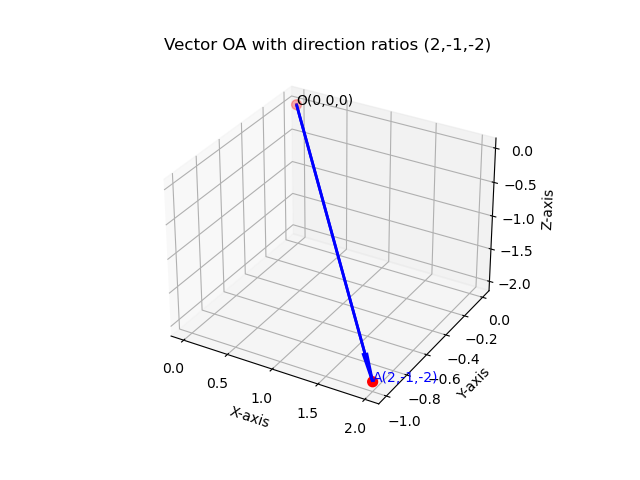
\includegraphics[width=0.8\columnwidth]{figs/fig_vector.png} 
   \caption*{Fig : Vector a}
  \label{Fig1}
\end{figure}

\end{frame}

\section*{Appendix: Code}

% C program
\begin{frame}[fragile]{C Code: points.c}
\begin{lstlisting}[language=C]

#include <stdio.h>

int main() {
  FILE *fp;

  // Endpoint of the vector with direction ratios (2, -1, -2)
  int x = 2, y = -1, z = -2;

  // Save origin and endpoint into file
  fp = fopen("points.dat", "w");
  fprintf(fp, "%d,%d,%d\n", 0, 0, 0); // Origin
  fprintf(fp, "%d,%d,%d\n", x, y, z); // Endpoint
  fclose(fp);

  return 0;
}

\end{lstlisting}
\end{frame}

% Python calling C
\begin{frame}[fragile]{Python: call\_c.py}
\begin{lstlisting}[language=Python]

import subprocess

# Compile C program
subprocess.run(["gcc", "points.c", "-o", "points"], check=True)

# Run the compiled program
subprocess.run(["./points"], check=True)

\end{lstlisting}
\end{frame}

% Python plotting
\begin{frame}[fragile]{Python: plot.py}
\begin{lstlisting}[language=Python]

import numpy as np
import matplotlib.pyplot as plt

# Load points from file
points = np.loadtxt("points.dat", delimiter=',')
x, y, z = points[:,0], points[:,1], points[:,2]

fig = plt.figure()
ax = fig.add_subplot(111, projection='3d')

# Plot points O and A
ax.scatter(x, y, z, color="red", s=50)  
ax.text(0, 0, 0, "O(0,0,0)", color="black")
ax.text(x[1], y[1], z[1], f"A({int(x[1])},{int(y[1])},{int(z[1])})", color="blue")

# Draw line OA
ax.plot([x[0], x[1]], [y[0], y[1]], [z[0], z[1]], color="blue", linewidth=2)

# Add arrowhead at A
ax.quiver(x[0], y[0], z[0], x[1], y[1], z[1],
          color="blue", arrow_length_ratio=0.1, linewidth=2)

# Axis labels
ax.set_xlabel("X-axis")
ax.set_ylabel("Y-axis")
ax.set_zlabel("Z-axis")
ax.set_title("Vector OA with direction ratios (2,-1,-2)")

# Save and show
plt.savefig("fig_vector.png")
plt.show()

\end{lstlisting}
\end{frame}

\end{document}
